% Pursuing Stacks (cotes 134-2 to 134-8): archive cote 134-3, site page 71 (PDF page 72), typescript page 71.
% typescript. Draft compared: ps2.tex:3667-3729.
% AI-transcribed by Claude Opus 5.5 (claude-opus-5-5, adaptive thinking, effort high), Message Batches API, batch ps1 (msgbatch_01Rv5hCaNTtUt4JHx1yqoHPL), 2026-11-12; image review recorded in records/CHECK_DECISIONS_134_3_4.tsv.
\scanpage{134-3/71}
\mspage{71}
having a closer look at \deleted{functors} \inserted{maps} f: $\over{B}{B}^{\deleted{\illegible{1}}}\hand{\to}$ A in (Cat) which are ``universal
\margin{X awkward}weak equivalences'' i.e. $W_{(\mathrm{Cat})}$ -aspheric\inserted{(46)}, namely such that for \uline{any} map
in (Cat) $A'\hand{\to}A$ (not only a localization\deleted{x} $A_{/a}\hand{\to}A$), the induced
functor $B'=B\mathrm{x}_A A'\hand{\to}A'$ is a weak equivalence. This property is a lot
stronger than just asphericity, and reminds of the ``trivial fibrations''
in Quillens theory. The usual criterion af asphericity for $B'\hand{\to}A'$ shows
that f is W-aspheric iff \deleted{if} for any A' with final element, and any func-%
tor $A'\hand{\to}A$, the fiber product $B'=B\mathrm{x}_A A'$ is aspheric. T\over[typed]{h}{h}e feeling here is
(suggested partly by Quillen's terminology) that this property is tied up
some way with the property for f to be a fibering(or cofibering ?) functor,
in the sense of fibered and cofibered categories, with aspheric fibers
moreover. Presumably fibered or cofibered categories \inserted{[in the purely categorical sense]}, with``base change
functors'' which are weak equivalences, will play the part of Serre-Quil-%
len's fibrations - and it is still to be guessed what kind of \deleted{categorical}
properties of a functor will play the part of \uline{co}fibrations. Apparently
they will have to be a lot more stringent than just monomorphisms in (Cat),
cf. \deleted{p. 37.} \hand{Section 30 [and (9)]}.

\margin{\diagram{\begin{tikzpicture}\draw[->] (.6,0)--(.2,0) .. controls (0,0) and (0,.2) .. (0,.4)--(0,1.3);\end{tikzpicture}}}H\over[typed]{e}{o}\over[typed]{w}{w}ever I feel it is not time yet to dive into the homotopy theory
properties of the all-encompassing basic modelizer (Cat), but rather come
back to the study of general (and less gene\over[typed]{f}{r}al) test categories.

\margin{\diagram{\begin{tikzpicture}\draw[->] (.6,1.3)--(.2,1.3) .. controls (0,1.3) and (0,1.1) .. (0,.9)--(0,0);\end{tikzpicture}}}41. One comment \inserted{still,} upon the role played in the theory I am developping of
the \hand{``}assumption\hand{''}(p.30) that the category of autoequivalences of (Hot) is
equivalent to the final category. This assumption has been a crucial
guide for putting the emphasis where it really belongs, namely upon
the set \deleted{of} $W\hand{\subset}\mathrm{Fl}(M)$ of weak equivalences within a category M which one
would like to take in some sense as a category of models for homotopy
types - the functors $M\hand{\to}$(Hot) following along auto\over[typed]{h}{m}atically. However,
in no statement whatever I proved so far, was this assumption ever used\over{.}{!}
\deleted{However,}\inserted{On the other hand,} the notion of a \uline{modelizer} introduced in the wake of the \hand{``}assumpti-%
on\hand{''} (cf. \hand{\S.28}) was tacitly changed during the reflection, by drapping al-%
together the condition a) of (strong) saturation of W, namely that W is
just the set of arrows\unsure{\hand{,}} made invertible by the localization functor $M\hand{\to}W^{-1}M$.
Instead of this, it turned out that the saturation condition we really had
at hands and which \xout{were} was adequate for working, was the conditions
a) to c) I finally wrote 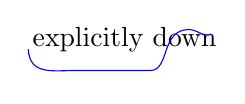
\begin{tikzpicture}[baseline=(t.base)]\node[anchor=base west,inner sep=0pt] (t) at (0,0) {explicitly down};\draw[color=blue] (-.05,-.03) .. controls (-.03,-.36) and (.25,-.30) .. (.55,-.30)--(1.50,-.30) .. controls (1.75,-.30) and (1.63,.22) .. (1.99,.22) .. controls (2.10,.22) and (2.17,.12) .. (2.28,.16);\end{tikzpicture} yesterday (\hand{\S.37}). As for the
strong saturation condition, for the time being (using nothing but what
has actually be\inserted{en} proved\deleted{\illegible{1}} so far, without reference to ``well known facts''
from homotopy theory)\hand{,} it is not even clear that the basic modelizer
(Cat) is one in the initial sense, namely that the set of weak equivalen-
